\begin{frame}{Selección de la Interfaz USB}
	\alert<2>{Cypress FX2LP}
	\begin{columns}
		\begin{column}{.4\textwidth}
			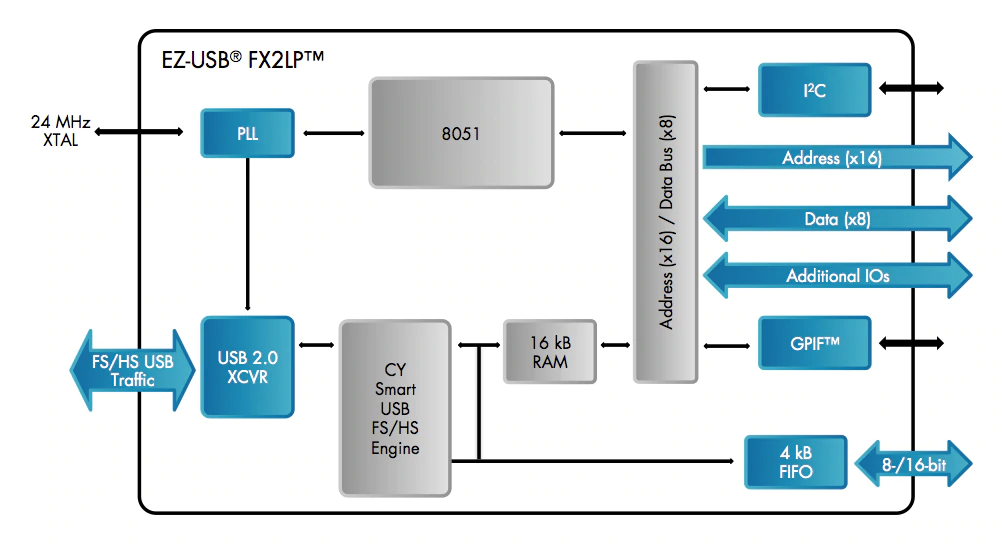
\includegraphics[width=\textwidth]{fx2lp}
		\end{column}
		\begin{column}{.6\textwidth}
			\begin{itemize}
				\item Pros
				\begin{itemize}
					\item Comunicación paralela de 16 bits
					\item Microcontrolador 8051
				\end{itemize}
				\item Contras
				\begin{itemize}
					\item Requiere esfuerzo en la configuración y software dedicado
				\end{itemize}
			\end{itemize}
		\end{column}
	\end{columns}
		
	FTDI FT4222H
	\begin{columns}
		\begin{column}{.4\textwidth}
			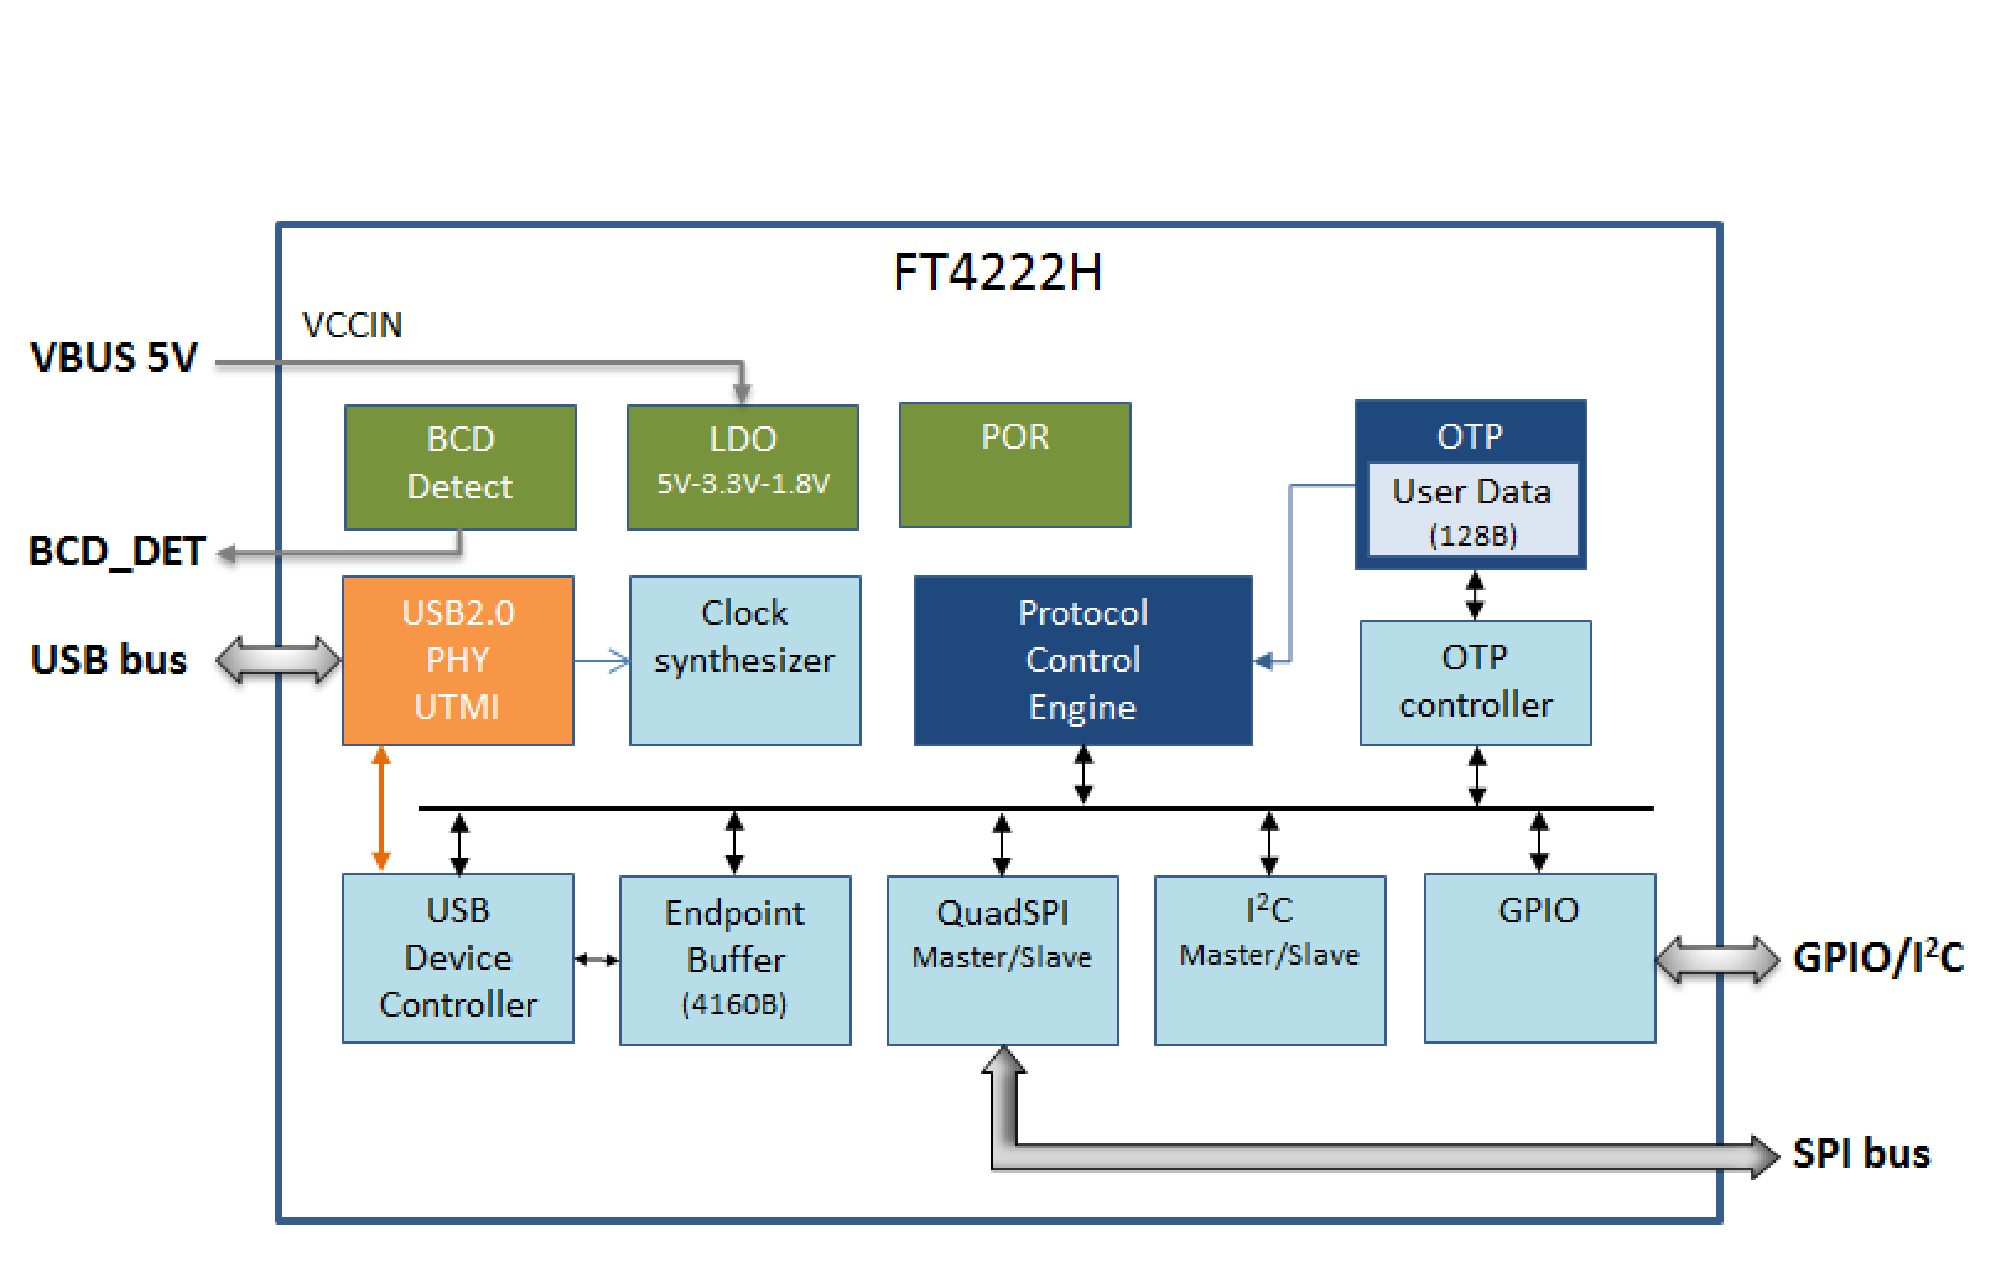
\includegraphics[width=\textwidth]{ft4222h}
		\end{column}
		\begin{column}{.6\textwidth}
			\begin{itemize}
				\item Pros
				\begin{itemize}
					\item No requiere programación
					\item Económico
				\end{itemize}
				\item Contras
				\begin{itemize}
					\item Solo permite Transferencias en Masa
					\item Comunicación SPI cuádruple
				\end{itemize}
			\end{itemize}
		\end{column}
	\end{columns}
\end{frame}

\begin{frame}{Selección del FPGA}
	\centering
	\begin{tikzpicture}[scale=1,>=latex]
		\begin{scope}[transform shape,node distance=2]
			\node[bloque]	(cy)				{Interfaz\\\alert{Cypress\\FX2LP}};
			\node[bloque]	(fpga)	[right=of cy]{FPGA};
			\node[bloque]	(pc) 	[left=of cy]	{PC};
			\draw[->,thick] (pc.15) -- node (usbd+) [above]	{D+} (pc.15 -| cy.west);
			\draw[->,thick] (cy.195) -- node (usbd-) [below]	{D-} (cy.195 -| pc.east);
			\draw[<->,thick] (cy.15) -- node (data) [above] {Datos} (cy.15 -| fpga.west);
			\draw[->,thick]  (fpga.195) -- node (ctrl) [below] {Control} (fpga.195 -| cy.east);
			\node[node distance=.4,text=blue] (usb text) [above=of usbd+] {USB};
		\end{scope}
		\begin{scope}
			\node[rectangle,rounded corners,draw=blue,dashed,fit=(usb text)(usbd+)(usbd-)(cy.south west)(pc.east)](usb){};
		\end{scope}
		\begin{scope}
			\node[draw=blue,ultra thick, ellipse,fit=(fpga)]{};
		\end{scope}
	\end{tikzpicture}
\end{frame}

\begin{frame}{Selección del FPGA}
	\begin{columns}
		\begin{column}{.28\textwidth}
			\centering
			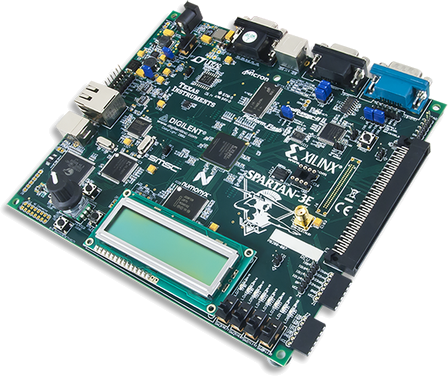
\includegraphics[width=\textwidth]{s3eboard}\\
			\centering
			Spartan-3E Starter\\
			\begin{itemize}
				\item FPGA Spartan 3E de Xilinx
				\item Gran cantidad de periféricos
			\end{itemize}
		\end{column}
		\begin{column}{.28\textwidth}
			\centering
			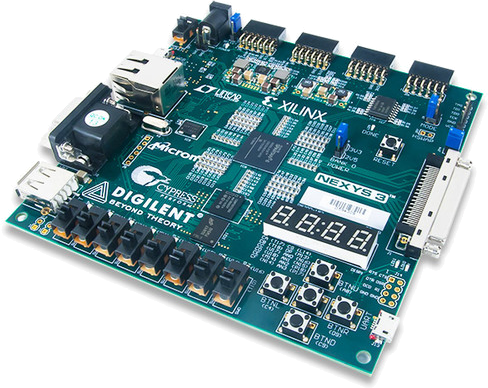
\includegraphics[width=\textwidth]{nexys3}\\
			\centering
			Nexys 3\\
			\begin{itemize}
				\item FPGA Spartan 6 de Xilinx
				\item Gran cantidad de periféricos
			\end{itemize}
		\end{column}
		\begin{column}{.28\textwidth}
			\centering
			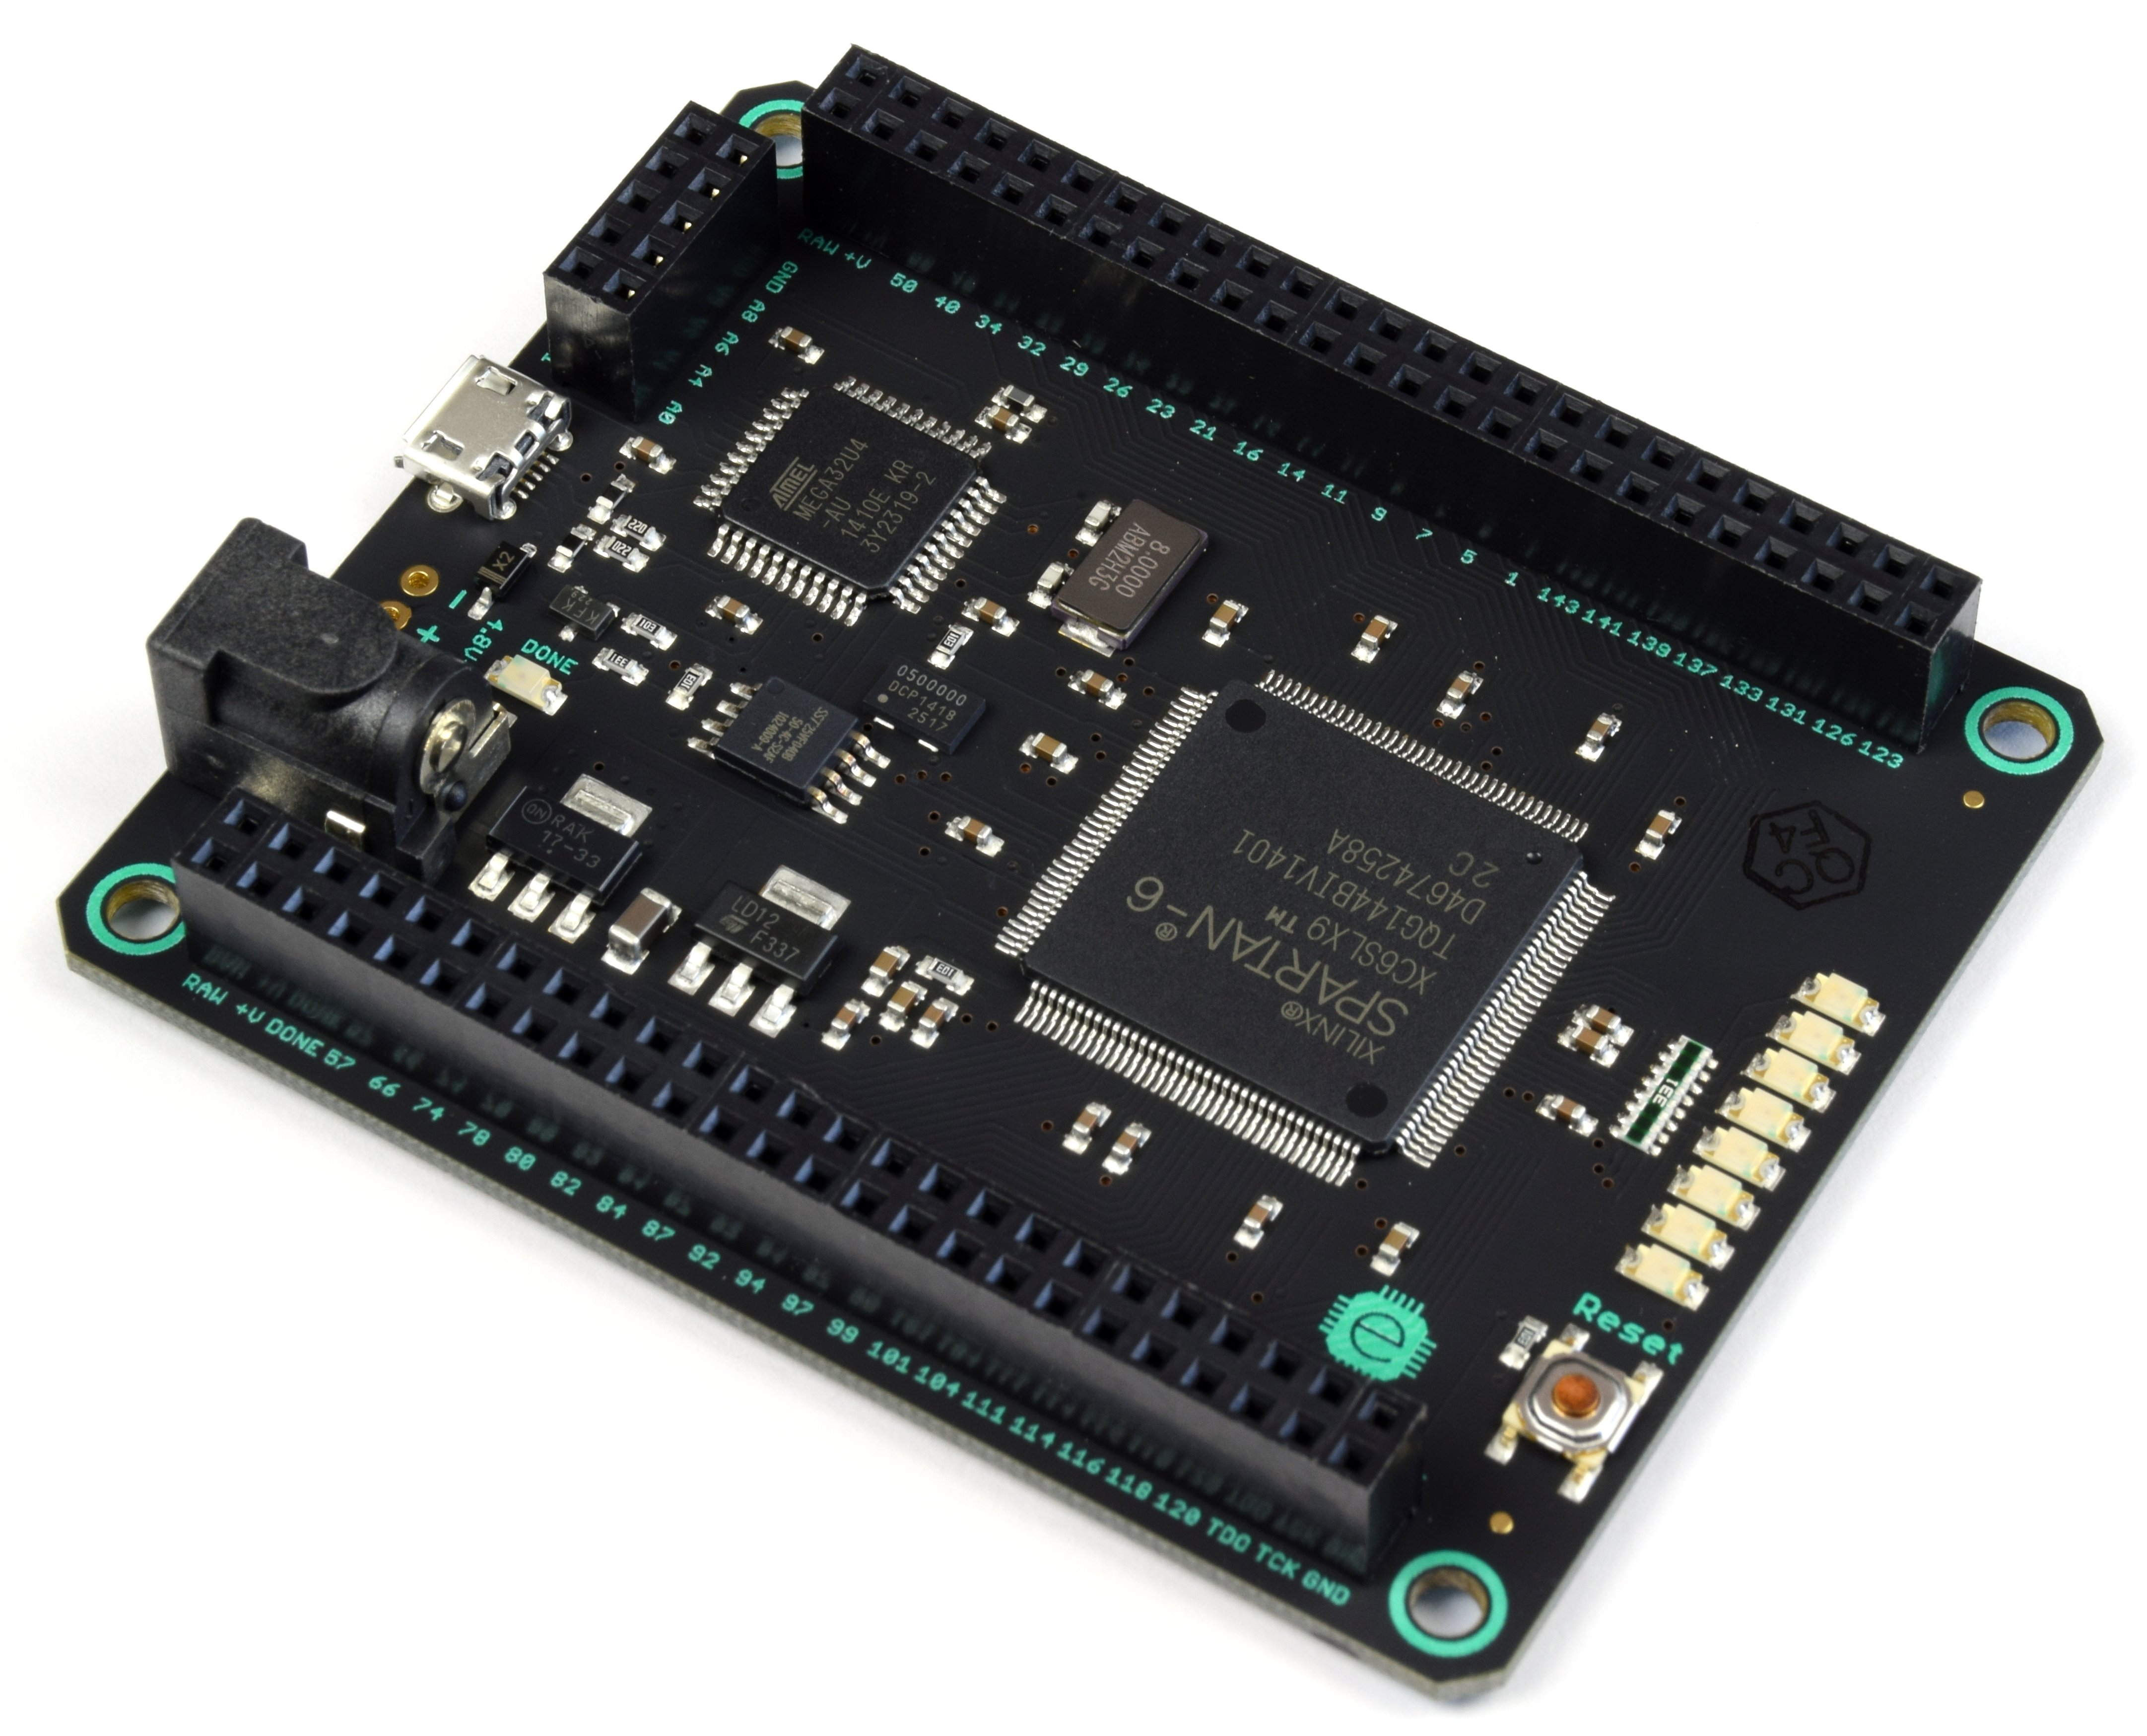
\includegraphics[width=\textwidth]{MojoIso}\\
			\centering
			\alert<2>{Mojo v3\\}
			\begin{itemize}
				\item FPGA Spartan 6 de Xilinx
				\item Muy económica
			\end{itemize}
		\end{column}
	\end{columns}
\end{frame}

\begin{frame}{La placa de desarrollo MOJO v3}
	\begin{columns}
		\begin{column}{.43\textwidth}
			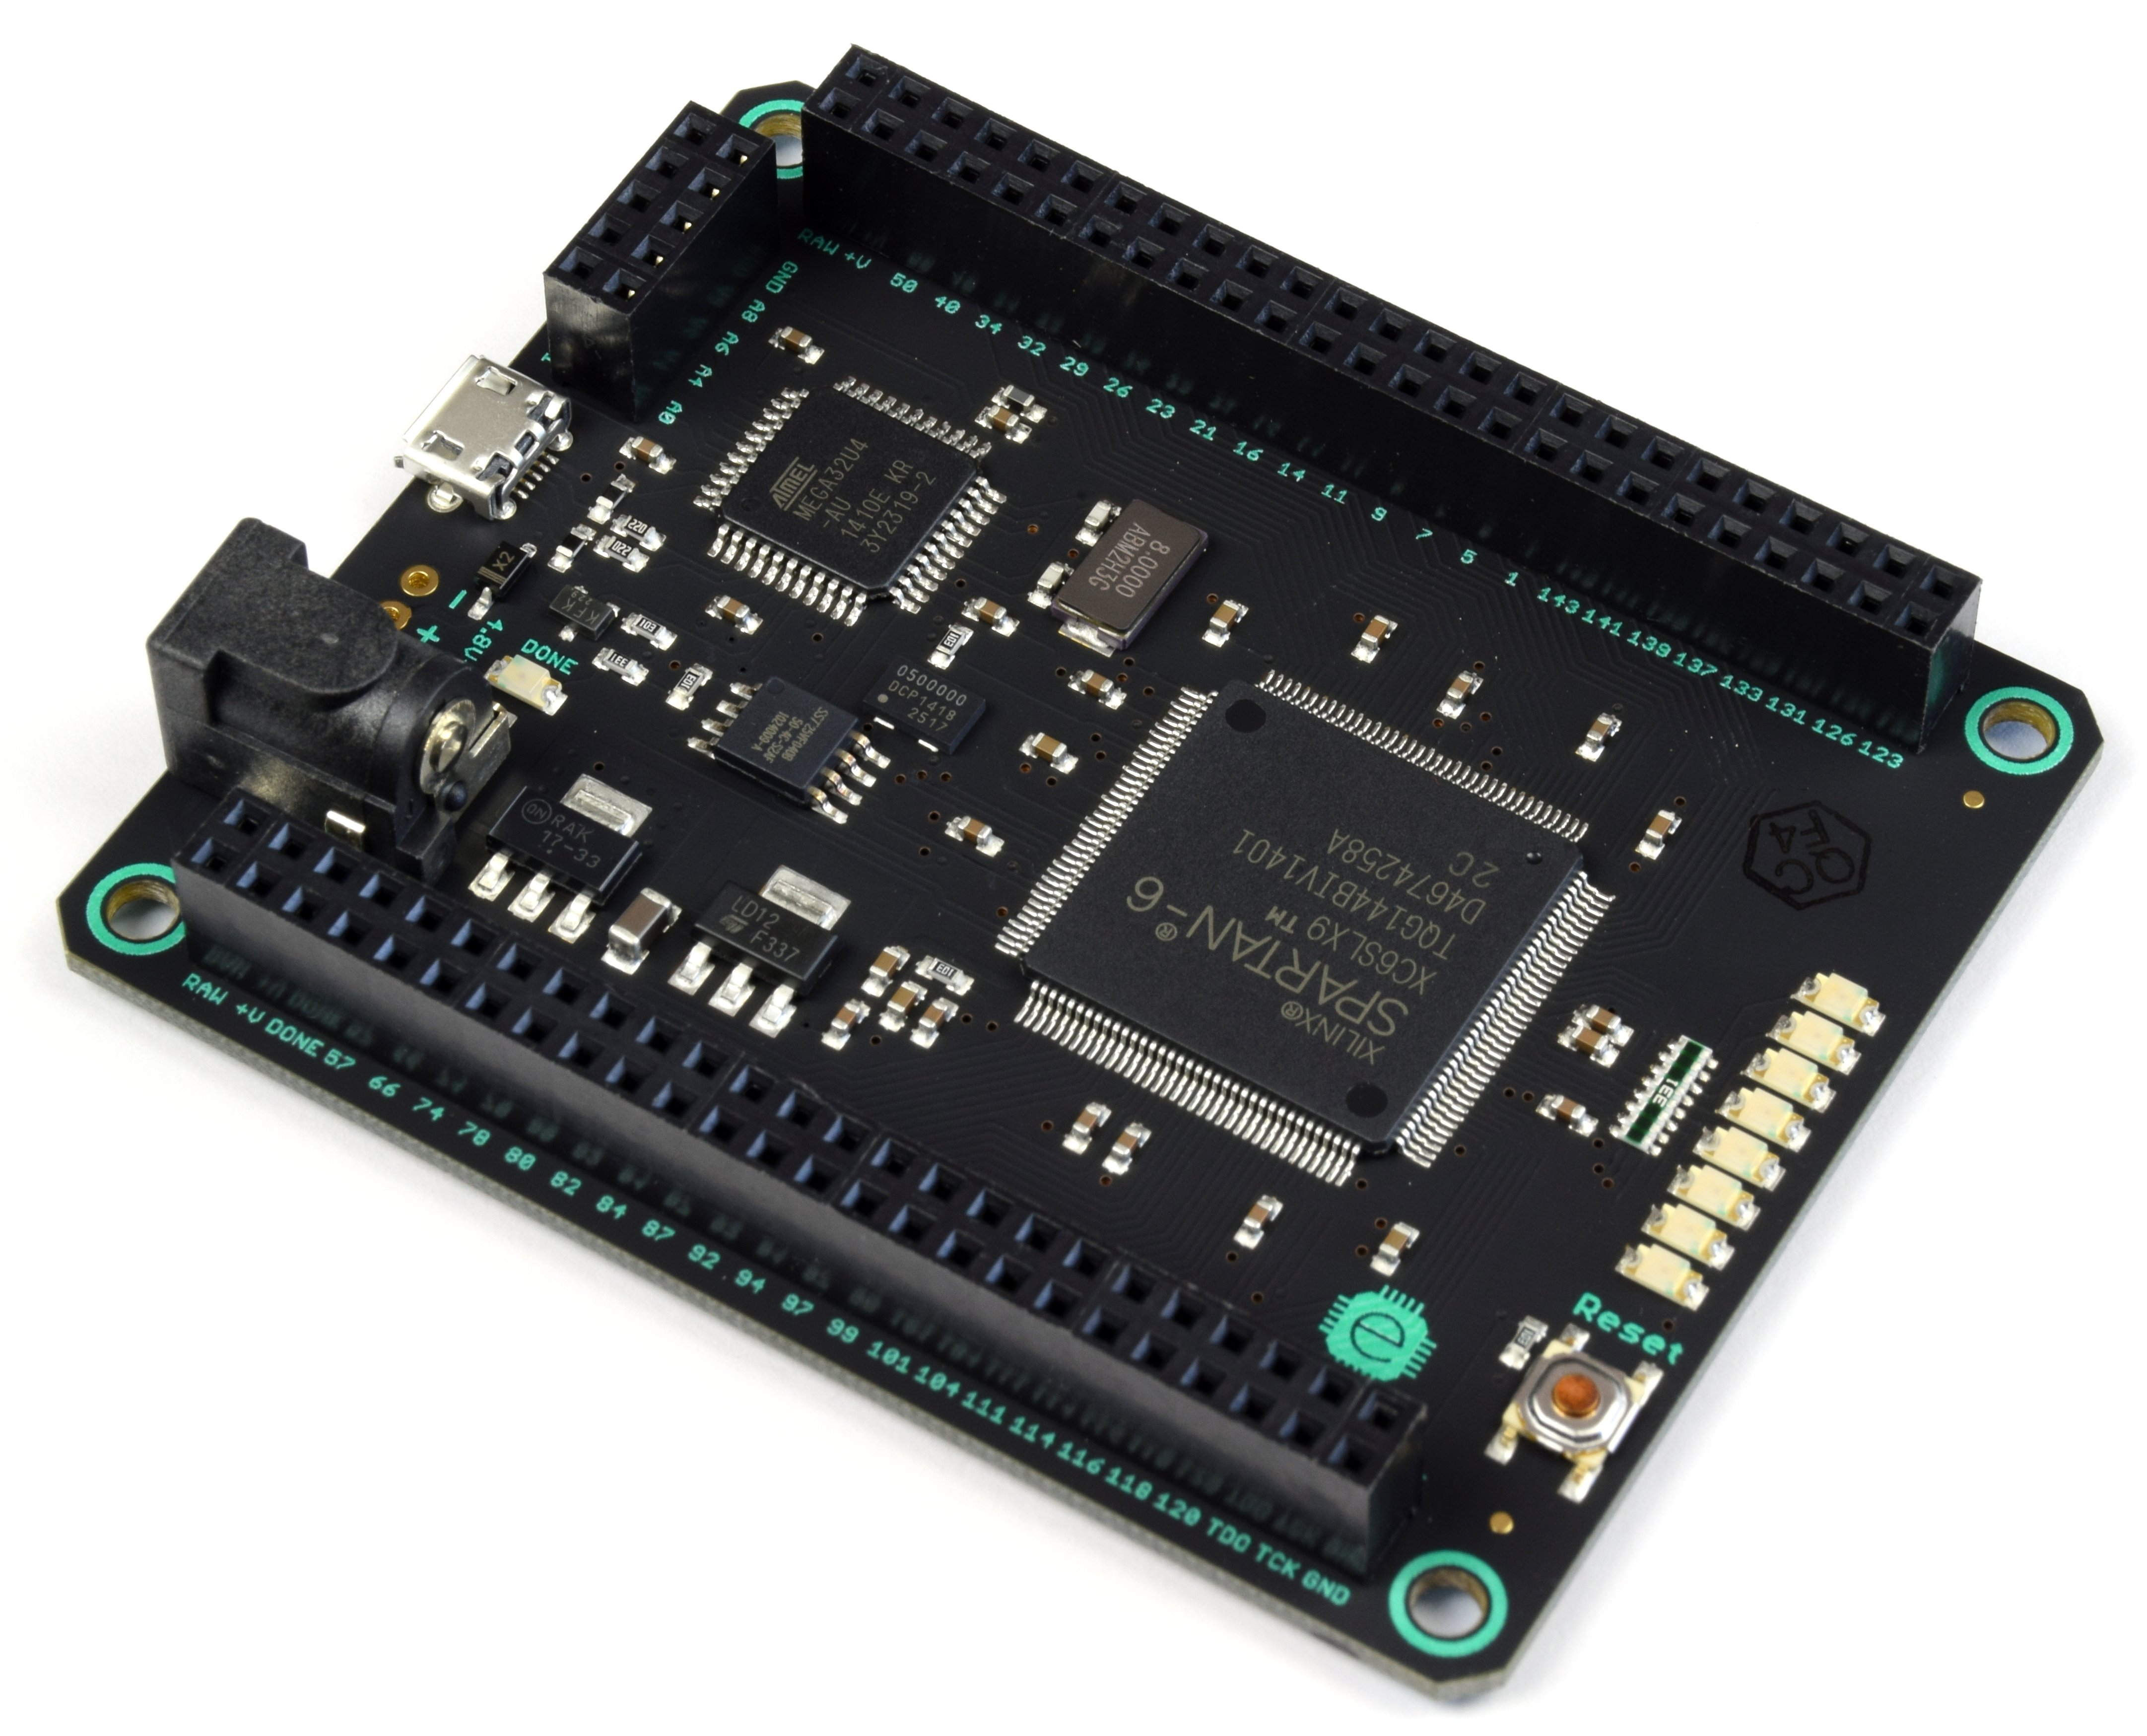
\includegraphics[width=\textwidth]{MojoIso.png}
		\end{column}
		\begin{column}{.55\textwidth}
			\begin{itemize}
				\only<1>{
					\item FPGA Spartan 6 XC6SLX9 de Xilinx
					\item 84 pines IO digitales
					\item 8 entradas analógicas
					\item 8 LEDs de propósito general
					\item 1 pulsador de propósito general
					\item ATmega32U4 para configurar la FPGA y leer los pines analógicos.
					\item Memoria flash para almacenar la configuración de la FPGA.}
				\item USB para programación y comunicación.
				\only<2>{
					\begin{itemize}
						\item USB 2.0 Full-Speed de 12 Mbps
						\item Implementado a través de controlador ATmega32U4
						\item Interfaz FPGA-ATmega32U4 via SPI de 8 Mbps.
					\end{itemize}
				}
			\end{itemize}
		\end{column}
	\end{columns}
\end{frame}

\begin{frame}{Circuito de interconexión}
	\begin{tikzpicture}[scale=1,>=latex]
		\begin{scope}[transform shape,node distance=2]
			\node[bloque]	(cy)				{Interfaz\\\alert{Cypress FX2LP}};
			\node[bloque]	(fpga)	[right=of cy]{FPGA\\\alert{Xilinx Spartan VI}};
			\node[bloque]	(pc) 	[left=of cy]	{PC};
			\draw[->,thick] (pc.15) -- node (usbd+) [above]	{D+} (pc.15 -| cy.west);
			\draw[->,thick] (cy.195) -- node (usbd-) [below]	{D-} (cy.195 -| pc.east);
			\draw[<->,thick] (cy.15) -- node (data) [above] {Datos} (cy.15 -| fpga.west);
			\draw[->,thick]  (fpga.195) -- node (ctrl) [below] {Control} (fpga.195 -| cy.east);
			\node[node distance=.4,text=blue] (usb text) [above=of usbd+] {USB};
			\node[node distance=.5,text width=60,align=center,text=blue] (pcb text)[above=of data]{Placa de\\Interconexión};
		\end{scope}
		\begin{scope}
			\node[rectangle,rounded corners,draw=blue,dashed,fit=(usb text)(usbd+)(usbd-)(cy.south west)(pc.east)](usb){};
			\node[rectangle,rounded corners,draw=blue,ultra thick,fit=(cy.south east)(fpga.north west)(pcb text)](pcb){};
		\end{scope}
	\end{tikzpicture}
\end{frame}

\begin{frame}{Circuito de interconexión}
	\only<1>{
		\begin{itemize}
			\item Versión 1:
		\end{itemize}
		\centering
		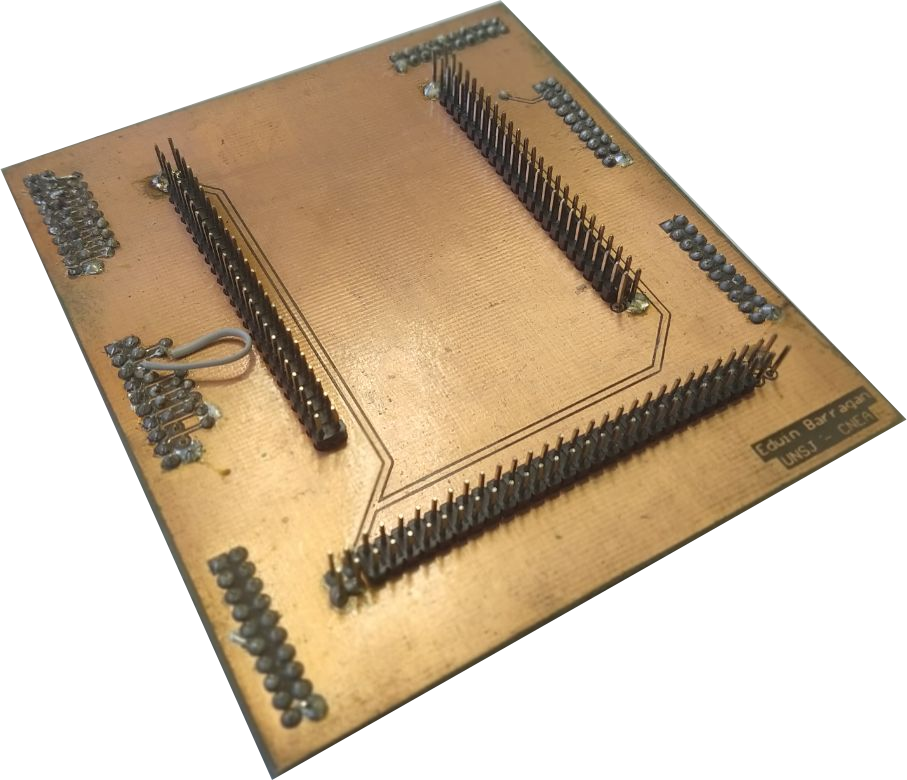
\includegraphics[width=.45\textwidth]{63v2anverso}
		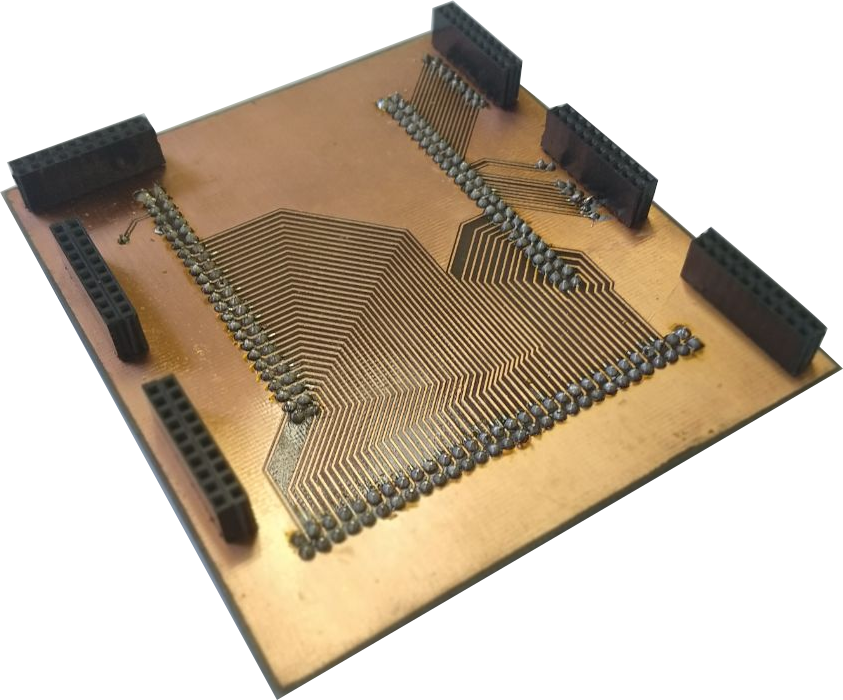
\includegraphics[width=.45\textwidth]{64v2reverso}
	}
	\only<2>{
		\begin{itemize}
			\item Versión 2:\\
		\end{itemize}
		\centering
		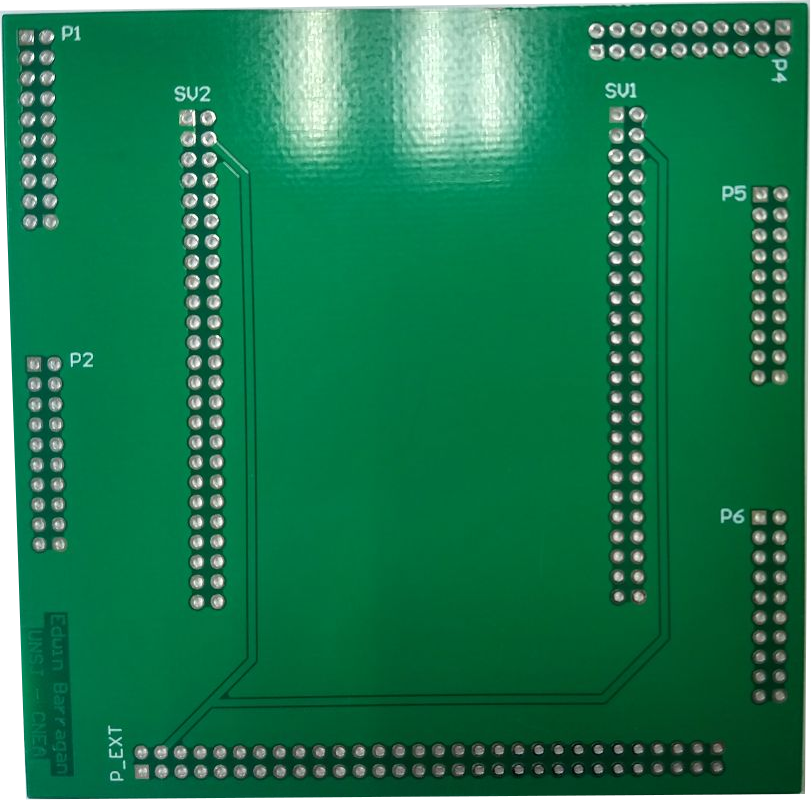
\includegraphics[width=.45\textwidth]{65v3anverso}
		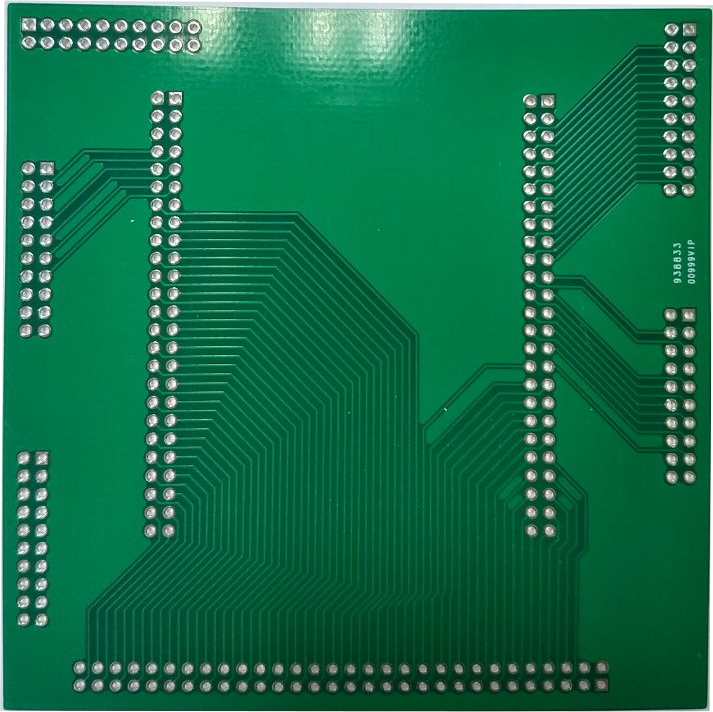
\includegraphics[width=.45\textwidth]{66v3reverso}
	}
\end{frame}

\begin{frame}{Componentes conectados}
	\centering
	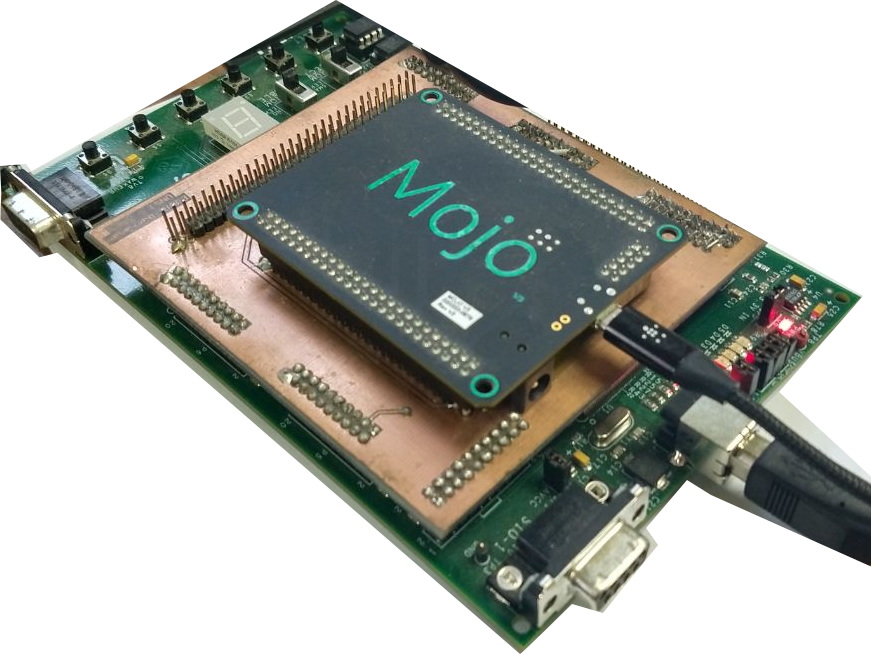
\includegraphics[width=.6\textwidth]{fisico}
\end{frame}

\begin{frame}{Acceso al dispositivo desde la PC}
	\begin{tikzpicture}[scale=1,>=latex]
		\begin{scope}[transform shape,node distance=2]
			\node[bloque]	(cy)				{Interfaz\\\alert{Cypress FX2LP}};
			\node[bloque]	(fpga)	[right=of cy]{FPGA\\\alert{Xilinx Spartan VI}};
			\node[bloque]	(pc) 	[left=of cy]	{PC};
			\draw[->,thick] (pc.15) -- node (usbd+) [above]	{D+} (pc.15 -| cy.west);
			\draw[->,thick] (cy.195) -- node (usbd-) [below]	{D-} (cy.195 -| pc.east);
			\draw[<->,thick] (cy.15) -- node (data) [above] {Datos} (cy.15 -| fpga.west);
			\draw[->,thick]  (fpga.195) -- node (ctrl) [below] {Control} (fpga.195 -| cy.east);
			\node[node distance=.4,text=blue] (usb text) [above=of usbd+] {USB};
			\node[node distance=.5,text width=60,align=center,text=blue] (pcb text)[above=of data]{Placa de\\Interconexión};
		\end{scope}
		\begin{scope}
			\node[rectangle,rounded corners,draw=blue,dashed,fit=(usb text)(usbd+)(usbd-)(cy.south west)(pc.east)](usb){};
			\node[rectangle,rounded corners,draw=blue,dashed,fit=(cy.south east)(fpga.north west)(pcb text)](pcb){};
			\node[ellipse,draw=blue,ultra thick, fit=(pc)]{};
		\end{scope}
	\end{tikzpicture}
\end{frame}

\begin{frame}{Acceso al dispositivo desde la PC}
	Para acceder al puerto USB desde la PC se utilizó la biblioteca libusb-1.0:
	\begin{itemize}
		\item Software libre: Puede ser utilizado sin necesidad de comprar una licencia.
		\item API portable: Permite escribir código que puede ser compilado en múltiples Sistemas Operativos.
		\item Abundante documentación: Se encuentran en Internet manuales y tutoriales muy completos sobre su funcionamiento.
	\end{itemize}
\end{frame}

\begin{frame}{Componentes del sistema}
	\begin{tikzpicture}[scale=1,>=latex]
	\begin{scope}
	\begin{scope}[transform shape,node distance=2]
	\node[bloque]	(cy)				{Interfaz\\\alert{Cypress FX2LP}};
	\node[bloque]	(fpga)	[right=of cy]{FPGA\\\alert{Xilinx Spartan VI}};
	\node[bloque]	(pc) 	[left=of cy]	{PC\\\alert{libusb}};
	\draw[->,thick] (pc.15) -- node (usbd+) [above]	{D+} (pc.15 -| cy.west);
	\draw[->,thick] (cy.195) -- node (usbd-) [below]	{D-} (cy.195 -| pc.east);
	\draw[<->,thick] (cy.15) -- node (data) [above] {Datos} (cy.15 -| fpga.west);
	\draw[->,thick]  (fpga.195) -- node (ctrl) [below] {Control} (fpga.195 -| cy.east);
	\node[node distance=.4,text=blue] (usb text) [above=of usbd+] {USB};
	\node[node distance=.5,text width=60,align=center,text=blue] (pcb text)[above=of data]{Placa de\\Interconexión};
	\end{scope}
	\begin{scope}
	\node[rectangle,rounded corners,draw=blue,dashed,fit=(usb text)(usbd+)(usbd-)(cy.south west)(pc.east)](usb){};
	\node[rectangle,rounded corners,draw=blue,dashed,fit=(cy.south east)(fpga.north west)(pcb text)](pcb){};
	\end{scope}
	\end{scope}
	\end{tikzpicture}
\end{frame}


